\documentclass{article}
\usepackage[utf8]{inputenc}
\usepackage[T1]{fontenc}
\usepackage[a4paper,top=3.5cm,bottom=3.5cm,left=2.5cm,right=2.5cm,marginparwidth=1.75cm]{geometry}
\usepackage{graphicx}
\usepackage[english]{babel}
\usepackage{multicol}
\usepackage{fancyhdr}
\usepackage{booktabs}
\usepackage{amsfonts, amssymb, amsmath, amsthm}
\usepackage{enumitem}
\usepackage{calrsfs}
\usepackage{hyperref}
\usepackage{cleveref}

\usepackage[labelfont=bf]{caption}


\pagestyle{fancy}
\lhead{MINES ParisTech}
\chead{S3 Research Internship}
\rhead{2019-2020}
\begin{document}

\newcommand{\spp}{superpixel}

\begin{center}
    \begin{Large}\textbf{IMAGE SEGMENTATION BY SUPERPIXELS}\end{Large}

    \vspace{1cm}
    \begin{large}\textbf{\underline{T.Dumont$^a$}, B.Figliuzzi$^b$}\end{large}

    \vspace{0.5cm}
    a. MINES ParisTech, theo.dumont@mines-paristech.fr\\
    b. MINES ParisTech CMM, bruno.figliuzzi@mines-paristech.fr
    \vspace{1cm}
\end{center}

\begin{center}
\noindent\textbf{Key-words: }\\
deep learning; convolutional neuronal networks; image segmentation\\
\ \\
\textbf{Abstract: }\\
In this paper, we study different options to improve the performance of a deep learning convolutional neuronal network
\end{center}

\tableofcontents

\section*{Todo}
\begin{itemize}
    \item
\end{itemize}

\newpage
\section{Introduction}

\subsection{Segmentation}
\paragraph{What it is}piche

\begin{figure}[!htb]
    \centering
    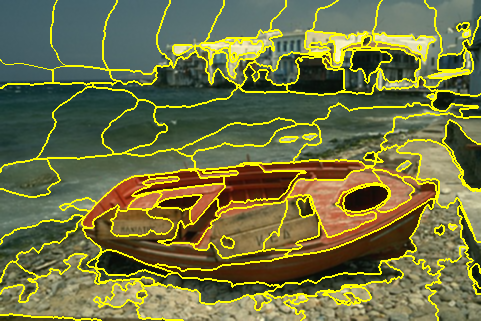
\includegraphics[scale=0.5]{img.png}
    \caption{\textit{An image and its segmented image}}
    \label{fig:segm}
\end{figure}
\paragraph{Motivation}

\subsection{Superpixels}
\paragraph{What it is}piche

\begin{figure}[!htb]
    \centering
    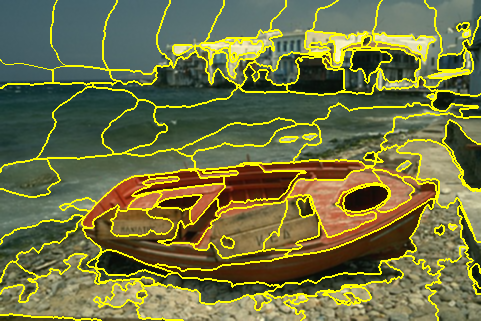
\includegraphics[scale=0.5]{img.png}
    \caption{\textit{Partition d'une image en superpixels}}
    \label{fig:spp}
\end{figure}

\paragraph{Applications \& Motivation}
démarrer une segmentation\\
fournir un support sur lequel faire de la classification (couleur/texture moyenne, etc)


\subsection{Ce qu'est une bonne \spp segmentation}
\paragraph{Métriques}
\paragraph{SLIC}
\paragraph{Autres algorithmes}

\subsection{Motivations/ambitions}
\paragraph{Difficultés que l'on cherche à résoudre}
\paragraph{Pas de vraie approche DL pour segmentation avec \spp s}
\paragraph{Ambitions}
améliorer les métriques


\section{Dataset generation}
\subsection{COCO dataset}
COCO dataset
\subsection{Eikonal}
\subsection{Notre utilisation de eikonal}
en plus réutilisé derrière sur image qui sort du réseau\\
faire un petit résumé

\section{Algo de ML}
\subsection{Approach}
description générale de l'approche (NN puis eikonal)
\subsection{Architecture}
\subsubsection{Chen}
structure\\
Dilated conv\\
ABN\\
LReLu
\subsubsection{Chen + Unet}

\subsection{Total Variation (TV) Loss}
\subsubsection{MSE}
\subsubsection{TV}
\paragraph{Formula}
\paragraph{Why}

est-ce que l'on parle de la façon dont on compute le gradient et des différentes méthodes que l'on a essayées

\subsection{Implementation}
The network was implemented with PyTorch\footnote{Code can be found at \url{https://github.com/theodumont/superpixels-segmentation}.} and we used GPU acceleration [...]
(pytorch), se renseigner (section assez courante)
GPU acceleraation
code sur github

\section{Expérience et résultats}
\subsection{Hyperparameters}
évolution des paramètres a et b ?\\
entrainement (lr, alpha) -> courbes de loss, et loss qui sature (cluster) d'où changement de lr au cours des epochs
\subsection{Results on dataset}


\section{Conclusion/Discussion}
On a présenté un nouveau...\\
On a prouvé...\\
Il reste à faire...

relire tous les mails pour avoir toutes les infos sur performances etc

\section*{Special thanks}

\section*{Sources}
\noindent{[}1] C. Smith, J.C. Green, Titre de l’article, Titre du journal, 10 (2009) 55-72\\
{[}2] M. Truk, C. Bidul. Titre du bouquin, John Wiley and Sons, New York, 1973\\
{[}3] P. Machin, Titre de la thèse, Thèse, Université Poitiers, 1992\\
{[}4] D. Pierre, J.-P. Paul, B. Jacques, Titre communication, in: D. Editor, G. Editeur, ( éd.), Proceedings of Conference XXX , Publisher, Paris, France, 1995, pp. 3–6

\end{document}
